
\section{Mental Clinic Simulation}

The basic architecture of \system~follows the universal LLM-based conversational agent~\cite{Park2023GenerativeAgents} setting, as Figure~\ref{fig:overview} illustrated. The main characters defined in the \system~can be divided into three parts: 
\begin{itemize}
    \item A variety of patients, generated based on existing patient portraits in D$^4$;
    \item Psychiatrist, the agent that reflecting skills based on the diagnosis conversation;
    \item Supervisor, an incomplete agent without long-term memory, acts as an optional plugin of the psychiatrist, initialized at the beginning of each session, mainly controlling the dialogue process and stimulating the psychiatrist agents to reflect on the diagnosis results.
\end{itemize}
%We will introduce the definition of different roles and their interactions here and the detailed agent structure will be described in \S~\ref{sec:method}.

\paragraph{Patient Agents}

Patient agents refer to agents playing individuals suffering from depressive moods and might be diagnosed with depressive disorder. They come to the clinic, seeking help from the psychiatrist agent to determine whether further intervention is necessary. To simulate depressive patients in a real-life scenario, we utilize a public quasi-clinical-standard depression diagnosis dialogue dataset D$^4$~\cite{yao-etal-2022-d4} to initialize patient agents, as step (1) in Figure \ref{fig:overview} represents. D$^4$ is a Chinese depression diagnosis dialogue dataset containing 1339 dialogues conducted by well-trained patients and psychiatrists. The data characteristics of the dataset are attached in the appendix. All the dialogues are collected based on portraits of real potential patients. We select 100 representative cases from the train set of D$^4$, two examples are shown in Figure~\ref{fig:portrait}. In the meantime, we also include the original 132 test cases in D$^4$ to conduct further experiments. Each selected case includes the patient profile, the dialogue history between the doctor and the patient, and the diagnosis result of the patient. \label{train/test}

To better simulate the symptom status of the patients, we adopt detailed symptom ontology defined in the Diagnostic and Statistical Manual of Mental Disorders (DSM-5-TR)~\cite{Arbanas2015DiagnosticAS} and prior work~\cite{Lan2024TowardsRA} to track the status of patients. However, patient agents are only provided with symptom lists, without the chief complaint and information about life events, resulting in poor role-play quality during the conversation, only replying whether they had the corresponding symptoms. Therefore, we use \texttt{GPT-4} to generate life event memory based on the dialogue history.

\paragraph{Psychiatrist Agent}
The psychiatrist agent is initialized with diagnosis skills from ICD-11\footnote{https://icd.who.int}. 
% The profile example is shown in Figure~\ref{fig:portrait}. 
It leads a conversation with patient agents, collecting information to be noted in the symptom list, as step (2) in Figure~\ref{fig:overview} illustrates. At the end of the session, the psychiatrist agent summarizes the electronic medical record (EMR) and diagnoses the depression risk and suicide risk of the patient agent. After receiving the reflected skills provided by the supervisor plugin and storing them in the memory, the psychiatrist agent calls for the next patient and repeats the diagnosis session, as step (5) and step (6) in Figure~\ref{fig:overview} represent. 


\begin{figure}[!t]
    \centering
    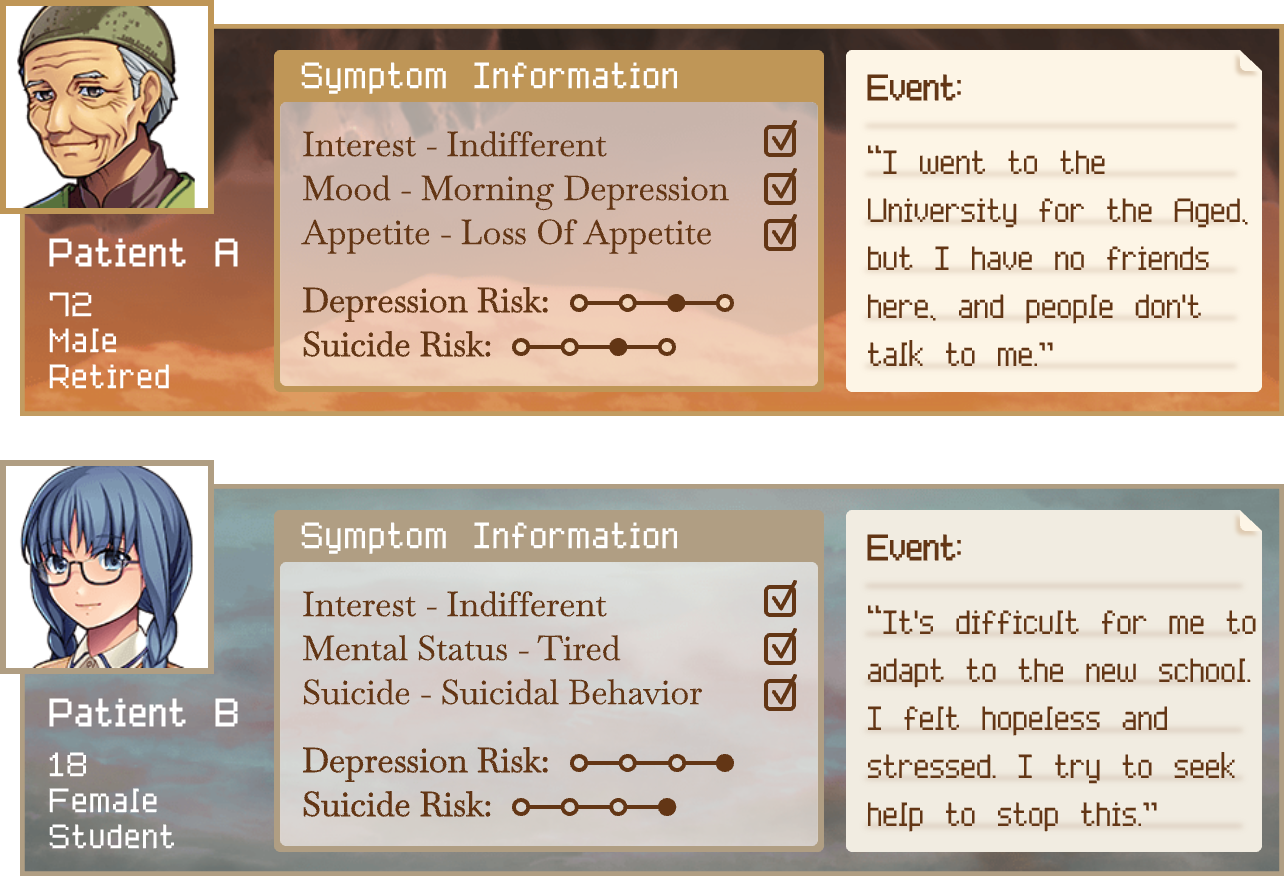
\includegraphics[width=1\linewidth]{fig/profile_v2.png}
    \caption{\textbf{Patient Profile Examples.}  We select two patient agents to illustrate. The profiles of patient agents are generated from cases of D$^4$.}
    % \caption{\textbf{Profile Examples.} The roles of agents are divided into patient and psychiatrist respectively. We select two patient agents and the psychiatrist agent to illustrate. The profiles of patient agents are generated from D$^4$ history, while the memory of the psychiatrist agent are collected from ICD-11.} %\MY{i don't think we need to show psychiatrist profile here, its icon image is also different from other figures, which is confusing}
    \label{fig:portrait}
\end{figure}


\paragraph{Supervisor Plugin}
The supervisor plugin acts as the coach or assistant of the psychiatrist agent, tracking the patient status and providing dialogue-controlling instructions during the diagnosis conversation, as step (3) in Figure \ref{fig:overview} shows. At the end of each session, the supervisor plugin compares the generated diagnosis results with the ground truth result diagnosed by a professional psychiatrist in D$^4$, reflects the skills that may be helpful to diagnose patients more precisely and provides them to the psychiatrist agent. We intentionally separate the supervisor as an individual role for future intervention from real psychiatrists, i.e. experts can intervene in the system to provide feedback and achieve a human-in-the-loop framework.
%\MY{I now get why you say it's a plugin, as you see it as a component of psychiatrist agent, consider moving it to an individual agent system?}